% Created 2020-08-15 Sat 03:26
% Intended LaTeX compiler: pdflatex
\documentclass[11pt]{article}
\usepackage[utf8]{inputenc}
\usepackage[T1]{fontenc}
\usepackage{graphicx}
\usepackage{grffile}
\usepackage{longtable}
\usepackage{wrapfig}
\usepackage{rotating}
\usepackage[normalem]{ulem}
\usepackage{amsmath}
\usepackage{textcomp}
\usepackage{amssymb}
\usepackage{capt-of}
\usepackage{hyperref}
\usepackage{graphicx}
\usepackage{longtable}
\usepackage{float}
\setlength{\parindent}{1em}
\setlength{\parskip}{0.5em}
\usepackage[citestyle=alphabetic,bibstyle=alphabetic, hyperref=true, backref=true,maxcitenames=3,url=true,backend=biber,natbib=true] {biblatex}
\addbibresource{bibliography.bib}
\usepackage[a4paper, total={7in, 9in}]{geometry}
\usepackage[ruled, procnumbered]{algorithm2e}
\usepackage{listings}
\SetArgSty{}
\usepackage[dvipsnames]{xcolor}
\usepackage{amssymb}
\usepackage{pifont}
\newcommand{\cmark}{\color{ForestGreen}\ding{52}}%
\newcommand{\xmark}{\color{Maroon}\ding{55}}%
\hypersetup{colorlinks=true}
\renewcommand{\sectionautorefname}{{\color{Black}\S}}
\renewcommand{\subsectionautorefname}{{\color{Black}\S\S}}
\renewcommand{\subsubsectionautorefname}{{\color{Black}\S\S\S}}
\renewcommand{\functionautorefname}{{\color{Black}\textbf{Function}}\color{Magenta}}
\renewcommand{\algorithmautorefname}{{\color{Black}\textbf{Algorithm}}\color{Magenta}}
\usepackage{subcaption}
\usepackage[shortlabels]{enumitem}
\usepackage{newfloat}
\DeclareFloatingEnvironment[fileext=lol, listname={List of Iterated Function System definitions}, name=IFS, placement=tbhp, within=section]{ifs}
\usepackage{wrapfig}
\usepackage{todonotes}
\usepackage{pifont,kantlipsum}
\newcommand*{\altasterism}{\vspace*{1em plus .5em minus .5em}\noindent\hspace*{\fill}\ding{104}\hspace*{\fill}}
\usepackage{rugscriptie}
\supervisor{dr. J. Kosinka}
\supervisor{G. J. Hettinga}
\date{August 2020}
\faculty{fwn} % Or feb, fgg, fgmw, fl, frg, frw, fw, umcg
\thesistype{Bachelors's thesis} % Will be printed unmodified
\author{Wiebe-Marten Wijnja}
\date{\today}
\title{\Huge In by Out again\\\medskip
\large Faking arbitrarily-deep zooming on Iterated Function Systems}
\hypersetup{
 pdfauthor={Wiebe-Marten Wijnja},
 pdftitle={\Huge In by Out again},
 pdfkeywords={},
 pdfsubject={},
 pdfcreator={Emacs 26.3 (Org mode 9.3.6)}, 
 pdflang={English}}
\begin{document}

\maketitle
\setcounter{tocdepth}{4}
\tableofcontents

\listoftodos


\section{Abstract}
\label{sec:orgbf73d8d}

Iterated Function Systems are a mathematical approach to rendering fractals that sees wide usage in the modeling of physical phenomena, 
image compression, and the creation of abstract art.
Current IFS rendering techniques meant that up to now, interactively exploring an IFS required fully re-approximating the IFS' attractor at every frame.

This thesis proposes a combination of two techniques to enable the faster exploring of IFSs.
First, a point cloud is used as intermediate attractor approximation, that can be re-used between animation frames.
Secondly, a technique coined 'self-similarity jumping' is employed to keep the attractor representation detailed, even when zooming in very far.

A proof-of-concept computer program was implemented which shows that the usefullness of the employed techniques, while promising, 
is hampered by the fact that self-similarity jumping cannot be used in a couple of common situations.

\section{Introduction}
\label{sec:org449267a}

Iterated Function Systems (IFSs) are a method to generate infinitely detailed fractal images 
by repeatedly applying simple mathematical functions until a fixed point is reached. \cite{barnsley2014fractals}
IFSs see use in rendering/modeling of physical phenomena, image compression \cite{hart1996fractal} and representing gene structures \cite{jeffrey1990chaos}.
Sometimes they also see use simply for the aesthetic beauty of their graphical representations \cite{draves2003fractal}.

Various computer algorithms to visualize IFSs exist \cite{hepting1991rendering}.
However, these all take either a still image as final result, or, if they want to render an animation,
view this as a sequence of separate still images to generate.

This leaves a door open for potential optimization: if there is information that remains the same between animation frames, 
then we could compute it only once and re-use this information for all frames.

For instance, many kinds of animations consist of transformations of the camera viewport w.r.t the viewed fractal over time like translation, rotation and scaling do not require alterations to the fractal itself.
This means that (an approximation of) the fractal might be computed once and then be used for all frames.

Furthermore, because of the self-similar nature of the rendered fractals,
it might it be possible to simulate zooming in to an arbitrary depth by 'jumping up' to a more shallow camera viewport
that shares the same self-similarity as the original one.

In this thesis, these two ideas are investigated in detail.

\subsection{Overview}
\label{sec:orge15cc62}

In the next section, \autoref{section:background}, Iterated Function Systems will be introduced and pre-existing methods to render their attractors in single-threaded and heavily parallel environments described.
This then leads to a clear definition of the research question in \autoref{section:research_question}.
The approach taken to test this question is described in \autoref{section:approach}, followed by qualitative results in \autoref{section:findings}.
We conclude in \autoref{section:conclusion} and finally hint at some approaches for further work in \autoref{section:further_work}


\section{Background}
\label{sec:orgbf93686}
\label{section:background}

This section will describe the different building blocks necessary to formalate the research question.
First, IFSs are formalized, followed by a description of the different ways in which an IFS' attractor can be rendered, 
and how these techniques might be paralellized.

\pagebreak

\subsection{Informal description of an Iterated Function System}
\label{sec:orge63dd7c}
\begin{figure}
\centering
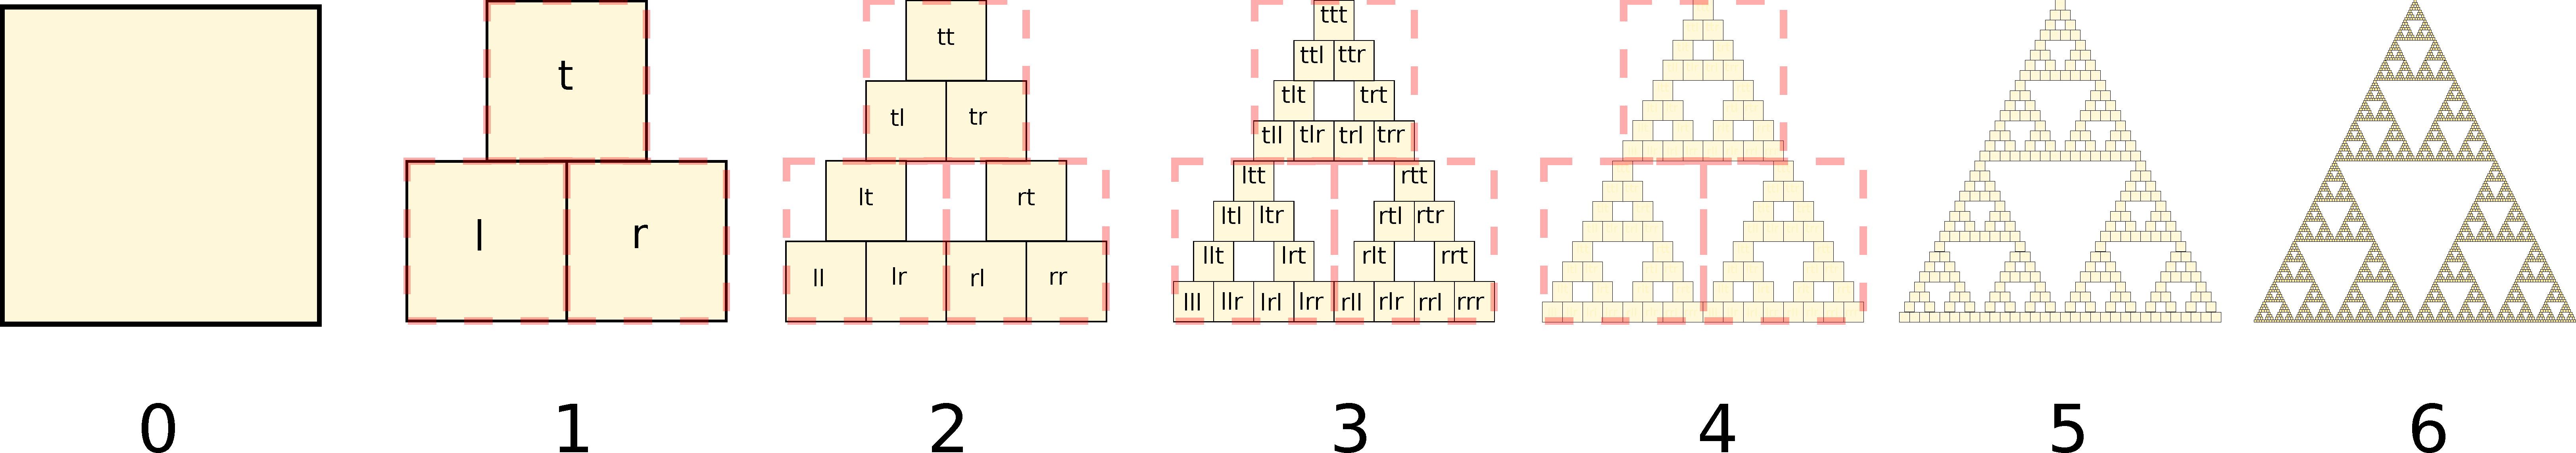
\includegraphics[width=\textwidth]{figures/sierpinsky_iterations}
\caption{The first six iterations of the Sierpi\'nsky triangle IFS (\autoref{ifs:sierpinsky}). 
The initial image is just the unit square. We then iteratively combine the results of transforming the current image using one of the three transformations. 
The letters indicate which (sequence of) transformation(s) resulted in this part of the image.
Dashed red lines are used for the first four iterations to indicate the self-similarity between the previous iteration and the current one extra clearly.
Even after a couple of iterations it can be seen that the shape of the original image does not matter for the shape of the attractor.}
\label{figure:sierpinsky_iterations}
\end{figure}


Informally, an Iterated Function System is a set of transformations that, given any input image, can create a new image by

\begin{enumerate}
\item transforming the input image with each of the transformations
\item combining all transformed images together. This is the new image.
\end{enumerate}

This process is then repeated an arbitrary number of times, until changes between the input image and output image are no longer visible to the human eye.

What you end up with is a visual representation of the IFS's attractor.
A simple example of this process can be seen in \autoref{figure:sierpinsky_iterations}

\todo[inline]{Some examples of IFSs? (that are used later on in the thesis)}


\subsection{Formal definition of an Iterated Function System}
\label{sec:org6bbb3c0}

Formally, an Iterated Function System consists of a finite set of contraction mappings that map a complete metric space \((\mathcal{M}, d)\) to itself:

$$ = \{ f_i : \mathcal{M} \rightarrow \mathcal{M} | i = 1, 2, \ldots, N \}, N \in \mathbb{N}$$

That each mapping needs to be contractive means that for each mapping \(f_i\), the distance between every two arbitrary points \(a\) and \(b\) in \((\mathcal{M}, d)\) needs to be larger than the distance of the points after transforming them:

$$d(f_i(a), f_i(b)) < d(a, b)$$

We can then take the union of performing all of these mappings on any compact set of points \(\mathcal{S}_0 \subset \mathcal{M}\). This procedure is called the \emph{Hutchkinson Operator} (\(H\)). 
We can iterate it as often as we'd like:

$$ \mathcal{S}_{n + 1} = H(\mathcal{S}_n) = \bigcup_{i=1}^{N} f_i(\mathcal{S}_n) $$

If we perform this operation an arbitrary number of times, we approach the fixed-point or attractor, \(\mathcal{A}\), of the Iterated Function System:

$$\mathcal{A} = \lim_{n \rightarrow \infty} \mathcal{S}_n$$

Curiously, which set of points \(\mathcal{S}_0\) we started with makes no difference (we might even start with a single point) \cite{mendivil2003fractals}.

\subsubsection{Restriction to affine transformations on the two-dimensional euclidean plane}
\label{sec:orgfce7251}

Most research of IFSs restricts itself to using \(\mathbb{R}^2\) as metric space\footnote{More formally, the two-dimensional Euclidean space: \(\left(\mathbb{R}^2, d(p, q) = \sqrt{p - q)^2}\right)\).} which can easily be rendered to screen or paper,
and furthermore most commonly-used IFSs are restricted to use \emph{affine transformations} as mappings.

Because of their prevalence, these are also the restrictions that will be used in this thesis.

\subsubsection{The viewport transformation}
\label{sec:orgf986d6f}
\label{subsection:viewport_transformation}

For any IFS with mappings we can transform its attractor by any invertible function \(t\) by adjusting each of the mappings according to the
transform theorem \cite{barnsley2014fractals} \(f_i' = t \cdot f_i \cdot t^{-1}\), essentially transforming points from the new space to the old space, then applying the mapping, and finally transforming them back to the new space. 
This allows us to give users freedom to choose any desired mappings and 'initial camera viewport' of the attractor,
while still allowing all calculations to happen with regard to the unit square (which keeps them simpler).

\subsection{Rendering an Iterated Function System}
\label{sec:org76381a2}

A couple of algoritms exist to render (visualize) the attarctor of an Iterated Function System. 
While it is impossible to render the attractor exactly, as this would require an infinite number of transformation steps,
we can approximate it until we are certain that the difference between our approximation and the attractor is smaller than
the smallest thing we can visually represent (e.g. smaller than the size of a pixel).

Because we apply \(H\) many times and each time consists of taking the union of \(N\) different transformations,
the result can be seen as traversing an (infinitely deep) tree of transformations, 
where each sub-tree is self-similar to the tree as a whole.

Different algorithms take different approaches to evaluating this tree (up to a chosen finite depth).

More in-depth information about the rendering of Iterated Function Systems can be found \cite{hepting1991rendering}. 
Short summaries of the two most common techniques will now follow.

\subsubsection{The deterministic method}
\label{sec:org49cfff6}

In this approach we evaluate the whole tree up to a chosen depth. The algorithm works as follows:

\begin{enumerate}
\item Pick a starting point \(z_0\);
\item Traverse the tree down to the chosen depth \(k\), building up a sequence of transformations \footnote{\(\circ\) stands for function composition: \((f \circ g)(x) = f(g(x))\). 
Be aware that when affine transformation functions are represented as matrices (e.g. \(F\) and \(G\)), matrix multiplication is in the opposite order (\(f \circ g \equiv G \cdot F\))}
\(f_{i_k} \circ \ldots \circ f_{i_1}\);
\item For each node at this depth, evaluate and render \(z_k = (f_{i_k} \circ \ldots \circ f_{i_1})(z_0) = f_{i_k-1}(z_{k-1})\);
\end{enumerate}

Since \(z_{k} = f_{i_k-1}(z_{k-1})\) this procedure takes, for an approximation that consists of \(N\) points, depending on the tree traversal chosen:

\begin{itemize}
\item a linear amount ( \(\mathcal{O}(N)\) ) of memory  for a breadth-first tree-traversal.
\item a logarithmic amount ( \(\mathcal{O}(\log{N})\) ) of memory for a depth-first tree-traversal.
\end{itemize}

The advantage of the breadth-first traversal is that generation could be stopped interactively,
while the depth-first traversal requires the stopping criterion to be known beforehand. \cite{hepting1991rendering}

While the deterministic method is easy to understand (and indeed is a direct translation of the informal process described at the start of \autoref{section:background}),
it is usually less efficient and more complex to implement on a computer than the algorithm that will be described next.

\subsubsection{The chaos game}
\label{sec:org94c5930}
\label{subsection:chaos_game}

\begin{figure}
     \centering
     \begin{subfigure}[b]{0.4\textwidth}
         \centering
         
\includegraphics[width=\textwidth]{figures/barnsley_1000000}
         \caption{1,000,000 points}
         \label{figure:barnsley_mil}
     \end{subfigure}
     \hfill
     \begin{subfigure}[b]{0.4\textwidth}
         \centering
         
\includegraphics[width=\textwidth]{figures/barnsley_100000000}
         \caption{10,000,000}
         \label{figure:barnsley_ten_mil}
     \end{subfigure}
        \caption{The Barnsley Fern, rendered using the chaos game with different amounts of points.}
        \label{figure:barnsley_chaos_game_points}
\end{figure}


The \emph{stochastic method} \cite{hepting1991rendering}, also known as the \emph{random iteration algorithm} \cite{barnsley2014fractals} or more frequently the \emph{chaos game}, works as seen in \autoref{chaosGame}

\begin{algorithm}[H]
\caption{the chaos game}
\label{chaosGame}
  $n$: the number of transformations the IFS consists of. \\
  $z$: a random point on the screen  \\
  \While{less than $N$ points plotted}{ 
    $i$: a random integer between $0$ and $n$.  \\
    $z = f_i(z)$  \\
    render($z$) except during the first $x$ iterations \\
  }

\end{algorithm}

This method converges to a correct result because of the following two facts:

\begin{itemize}
\item because the precision of the canvas we render on is finite, and because all transformations are contracting,
two points \(a\) and \(b\) are indistinguishable after only \(x\) transformations.
 In other words, only the latest \(x\) transformations determine at what location on the canvas a point will end up (with the latest transformation having the largest effect on the point's final location).\footnote{Methods for precisely determining the lower and upper bounds of IFS contraction for a particular IFS (and therefore the exact value of \(x\)) exist \cite{hepting1991rendering}, 
but are not relevant for this thesis.}
\item at each depth in the tree the subtree remains the same, so every sequence of transformations approaches the attractor.
\end{itemize}

Therefore, all intermediate points after the first \(x\) iterations are visually indistinguishable from the a point that is part of the attractor.
By running this non-deterministic approach for enough iterations we approach a diverse enough set of 'transformation sequences of length \(x\)' that we end up covering the whole attractor.

The nice thing about the chaos game is that it does not require any extra memory (besides the point \(z\)).
Also, because it is so simple and little auxiliary memory is needed, it runs very efficiently on modern CPU architectures.

A disadvantage of the chaos game is that the result is by its very nature \emph{non-deterministic}.
If not enough points are used, the result might end up 'grainy' and it is not predictable what part of the attractor will be covered (see \autoref{figure:barnsley_chaos_game_points}).


One further disadvantage the chaos game has, is that in its simplest form, all transformations have an equally likely chance to be used.
However, because some transformations might be (much) more contracting than others, this means that coverage of the attractor is not even,
which means that we need to use much more iterations than would be the case if we balance it out.

Therefore, most implementations of the chaos game allow (or require) the user to specify a \emph{probability} for each transformation.
All these probabilities together ought to sum up to 1.\footnote{These probabilities are often fine-tuned by hand, although algorithms to determine balanced probabilities exist as well \cite{hepting1991rendering}.}

\altasterism

Because of its simplicity and computational efficiency, the chaos game is used more frequently than the deterministic method for practical implementations.
The chaos game is also easier to paralellize for Graphical Processor Units (GPUs), as will be outlined in the next subsection.

\subsection{Paralellizing IFS rendering by using a Graphical Processor Unit}
\label{sec:orgf26de1e}

It is enticing to port IFS rendering to run on GPU-architecture because to produce a smooth image, often hundreds of millions of points are needed.

However, optimizing IFS rendering to run well on GPU-architectures is a bit of a challenge.

GPU shaders usually operate by running a check for every pixel on the final canvas, to determine its color.
For other fractals like the Mandelbrot- and Julia-sets, this is a natural fit since the construction of those fractals works exactly in that way.

For an IFS this does not work, as an IFS is created in the other direction. Points end up at some location on the canvas \emph{only after transforming} many times.
Attempts to go the other way fall flat, for instance because this would require to invert the IFS' mappings, but they are not guaranteed to be invertible.

Instead, General-Purpose GPU-techniques are used that are able to use the top-down approach.

\subsubsection{The chaos game on the GPU}
\label{sec:orge6ac5f7}
\label{subsection:chaos_game_gpu}

The deterministic method is difficult to paralellize on the GPU because of the extra memory that is required to keep track of the current position in the tree.
Coordinating which GPU thread would calculate which part of the tree and sharing results would be a hassle.

Instead, the chaos game is more frequently used because of its simplicity. It is paralellized in a straightforward way, by running the iteration process many times side-by-side (one per GPU thread),
and then combine the final results of all of these on a single canvas. \cite{green2005gpu}

\subsubsection{The deterministic method on the GPU}
\label{sec:org5b04555}
\label{subsection:deterministic_gpu}

An exciting approach taken in \cite{lawlor2012gpu} uses the deterministic method instead:
by using the fast inverse square root operation, even unbounded (noncontracting) and nonlinear IFSs can be efficiently
evaluated using the deterministic method, programmed in normal GPU shaders that manipulate a couple of GPU textures.


\section{Research Question}
\label{sec:orgc9da940}
\label{section:research_question}

In the last section, the construction of an IFS's attractor was formally defined, 
and different approaches of rendering it were outlined.

While many different approaches to IFS rendering exist, some of them quite efficient,
none of them re-uses information from rendering one image of the IFS for rendering another.

This leads us to the research question of this thesis:

\textbf{\textbf{Is it possible, by re-using information between animation frames, to render animations of an Iterated Function System's attractor in which the camera zooms in, in real-time?}}

\section{Approach}
\label{sec:orgba5c68e}
\label{section:approach}

To put this to the test, a simple software program was created which calculates the IFS' attractor only once,
and then allows a user to interactively zoom and pan the camera around to investigate different parts of the attractor.

\subsection{Design}
\label{sec:org60385e8}

The inspiration of the design is two-fold:

First, we use the insight that the (parallel) chaos game can be used to generate a \emph{point cloud}, allowing us to re-use parts of the computation between animation frames
and thus render each frames faster.

Second, while a point cloud only allows \emph{zooming in} up to a particular depth before losing considerable detail, 
it is possible to detect when we are looking at a self-similar part of the attractor.
This allows us, in many situations, to replace the current camera viewport with a more \emph{shallow} one, keeping the amount of detail high.

\subsubsection{Point clouds}
\label{sec:orge016262}

The main inspiration for the re-usability approach is that we can modify the GPU-variant of the chaos game algorithm outlined in \autoref{subsection:chaos_game_gpu}
to render to a \emph{point cloud} instead of immediately to a canvas.
When we then move around the camera, we are able to re-use the points in the point cloud;
only where the points in the point cloud end up on screen exactly needs to be re-calculated, 
by transforming all of the points exactly once with the 'view transformation' 
(and culling all points outside of the viewport).

This is faster than re-evaluating the whole attractor using the chaos game at every frame which would require transforming all points \emph{many} times.

Formally, to render an attractor approximation consisting of \(N\) points, 
running the whole chaos game each frame takes \(2(N+x)\) transformations per frame. \footnote{Using the definitions of \autoref{subsection:chaos_game}: \(N\) is the total number of points we want to render in our attractor approximation, 
and \(x\) is the minimum number of transformations we need to apply to any arbitrary point to make it visually indistinguishable from a point exactly on the attractor.} 
Running this on \(p\) parallel threads has a time complexity of \(\mathcal{O}(\frac{2(N+px)}{p})\).

Unoptimized, it takes \(N\) transformations to render a precomputed point cloud to screen each frame (in parallel this corresponds to a time complexity of \(\mathcal{O}(\frac{N}{p})\)).
This does not seem very impressive since \(\mathcal{O}(\frac{2(N+x)}{p}) \approx \mathcal{O}(\frac{2N}{p}) \approx \mathcal{O}(\frac{N}{p})\),
placing the two approaches in the same order of efficiency. However, it is possible to optimize point cloud-based rendering using the techniques outlined in the next section
to run in \(\mathcal{O}(\frac{\log{N}}{p})\) instead, which is a big improvement.

\subsubsection{Potential point cloud-based optimizations}
\label{sec:org017fd4b}
\label{subsection:point_cloud_optimizations}

The generation and rendering of point clouds is a quite well-understood problem \cite{wimmer2006instant}. point clouds see widespread use,
most commonly in 3D-graphics that originates from a '3D scanner' .

point clouds can be rendered in a reasonably efficient manner by storing them in a 'Bounding Volume Hierarchy',
for instance in a binary search tree that is ordered using the Morton space filling curve. \cite{lauterbach2009construction}
Storing the points of a point cloud in this way allows us to efficiently cull most uninteresting points (i.e. points that would end up outside of the current camera viewport),
which speeds up the rendering procedure tremendously.

However, while this problem is well-understood, the implementation is far from trivial \cite{lauterbach2009construction}.

\subsubsection{Detecting self-similarity: 'Zooming In by Zooming Out'}
\label{sec:orgd05001c}
\label{subsection:self_similarity}

When using a point-cloud, we retain detail when zooming in up to a certain depth. In this way, a point cloud is more flexible than a 
static pixel canvas, which will already show rendering artefacts when zooming in slightly beyond its intended size.
\todo[inline]{More info}

Nonetheless, beyond a certain depth, the number of points of the point cloud that fall outside of the current camera viewport
(and thus are 'useless' for the quality of the rendered attractor) grows larger and larger.

However, it follows from the self-similar nature of the IFS that we might, in certain situations,
'secretly' zoom out to a shallower camera viewport of the point cloud that shows the same information of the attractor
as the original viewport, but containing more points of the point cloud.

This can be done by identifying a mapping that fully encompasses the current camera viewport, and then applying its inverse
to the viewport.
'Fully encompasses' here means that the unit square transformed by the mapping fully encompasses
the unit square transformed by the inverse of the camera viewport transformation \footnote{A simple way to do this is to treat the unit square as a simple polygon,
and then transform all of its corner points. For the resulting two polygons, the 'even-odd rule' algorithm
\cite{haines1994point}
can be used to check whether all points of one polygon are inside the other.}.

\todo[inline]{Example picture}

\subsubsection{Coloring the rendering}
\label{sec:orgfa8677d}
\label{subsection:coloring}

The simplest way of rendering an IFS attractor simply renders points that are on the attractor a different colour
than the points that are not.

However, more visually pleasing methods use a \emph{color map} to e.g. indicate the density (the number of points ending up at a particular canvas location) of the attractor.
Yet more advanced methods \cite{draves2003fractal} keep track of a per-point colour, based on the sequence of transformations it has undergone.

It seems possible to combine these techinques with the 'self-similarity jumping', since we keep track of which mappings we've (inversely) applied to the camera viewport:
to determine the final colors of all points, all visible points need to be multiplied 
all points's colors need to be altered by the color-mutations that each of the inversely-applied mappings would apply.
Essentially, say we are viewing the lower left leaf of a fractal fern, whose mapping would make the contained points reddish. 
If we now 'jump up' (so we use points from virtually the whole fern), we have to alter all points so they get the same reddish hues.


\subsection{Implementation}
\label{sec:orgf632874}

\begin{figure}
  \centering
  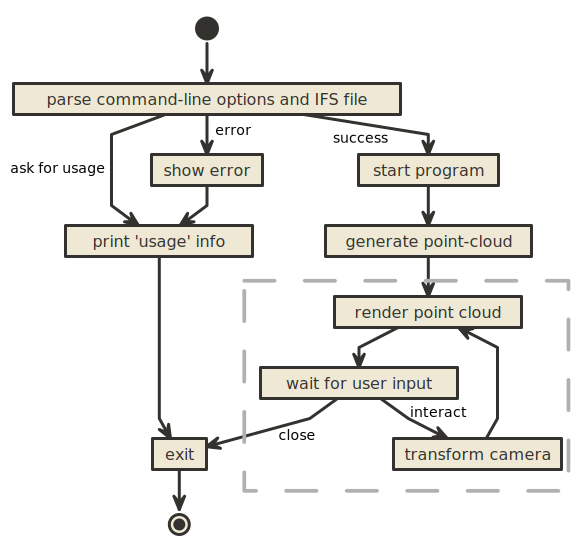
\includegraphics[width=0.5\textwidth]{figures/program_execution}
  \caption{Overview of the proof-of-concept program's execution flow.}
\label{figure:program_flow}
\end{figure}

The program was implemented using the general-purpose programming language Haskell, 
in combination with the GPGPU library Accelerate \cite{chakravarty2011accelerating}.
This programming stack was chosen because Accelerate 
offers a statically-typed EDSL\footnote{Embedded Domain-Specific Language.} to array-based GPGPU programming,
which is more high-level and less error-prone than writing shader code in e.g. CUDA or OpenCL directly.\footnote{Instead of being presented with a black screen when a programming mistake is made, 
Accelerate presents errors at compile-time in many cases. Furthermore, Accelerate features a
single-threaded reference implementation that runs on the CPU that can be used to sanity-check the behaviour of code.}

The usage of Haskell as implementation language also allowed 
the easy construction of different subcomponents making up the program,
and testing each of these independently, being a pure functional language.

A general overviwe of the flow of the program can be seen in \autoref{figure:program_flow}.

\subsubsection{Simplicity}
\label{sec:org5954dc1}

To be able to complete the implementation within the time allotted for the thesis project,
the decision was made to keep the implementation as simple as possible.

This means that 

\begin{itemize}
\item the optimizations mentioned in \autoref{subsection:point_cloud_optimizations} were not implemented.
\item points are rendered on screen using a simple binary mapping (if a pixel contains one or more points, it is white; otherwise black.)
the more fancy coloring techniques outlined in \autoref{subsection:coloring} were not used.
\end{itemize}

This means that while the program cannot on its own fully answer the question of whether
this technique is fast enough for real-time usage in all circumstances,
it is able to answer the simpler question of whether the technique of using a point cloud
in combination with 'self-similarity jumping' is at all feasible.

\subsubsection{Command-line options}
\label{sec:org9bdcc64}

The proof-of-concept program allows the customization of the following options

\begin{itemize}
\item `samples`: the number of points to use for the chaos game (defaults to 100,000,000)
\item `paralellism`: the number of GPU-threads to split the number of samples across. (defaults to 2048)
\item `seed`: a number to seed the random number generator with. If not provided, a different arbitrary seed will be used each time.
\item `render\_width` and `render\_height` set the resolution of the program window that is displayed (defaults to \(800 \times 800\)).
\end{itemize}

\subsubsection{`.ifs' file format}
\label{sec:org92b912e}

The configuration language 'Dhall' \cite{gonzalez2019} was used to 
easily faciltate the specification of different IFSs.

The file structure allows one to indicate a list of affine transformations with associated chaos game probabilities,
as well as an 'initial camera viewport transformation'. \autoref{subsection:viewport_transformation}

Dhall allows the definition and re-use of variables, which can be useful
for numerical constants that are used in multiple transformations.\footnote{Unfortunately, Dhall explicitly does not allow floating-point arithmetic.
As such, one still needs to write e.g. \(1/3\) as \(0.3333333333333333\).}

An example file can be seen in \autoref{listing:barnsley_fern_ifs_file} .


\begin{lstlisting}[float, language=Haskell, frame=single, breaklines=true, basicstyle=\scriptsize\tt, captionpos=b, caption={barnsley\_fern.ifs, representing \autoref{ifs:barnsley_fern}}, label={listing:barnsley_fern_ifs_file}]
{ initialCamera =
  { a = 9.090909090909091e-2
  , b = 0.0
  , c = 0.0
  , d = -9.090909090909091e-2
  , e = 0.5
  , f = 1.0
  }
, transformations =
  [ { transformation = { a = 0.0, b = 0.0, c = 0.0, d = 0.16, e = 0.0, f = 0.0 }
    , probability = 1.0e-2
    }
  , { transformation = { a = 0.85, b = 4.0e-2, c = -4.0e-2, d = 0.85, e = 0.0, f = 1.6 }
    , probability = 0.85
    }
  , { transformation = { a = 0.2, b = -0.26, c = 0.23, d = 0.22, e = 0.0, f = 1.6 }
    , probability = 7.0e-2
    }
  , { transformation = { a = -0.15, b = 0.28, c = 0.26, d = 0.24, e = 0.0, f = 0.44 }
    , probability = 7.0e-2
    }
  ]
}

\end{lstlisting}

\subsubsection{Rendering}
\label{sec:org4471ce4}
The program computes the point cloud once, on startup, and then re-renders the image that is shown in the program window
every time the user changes the camera viewport.

Rendering is done by iterating (in parallel) over all points in the point cloud and filling a two-dimensional histogram with the same dimensions
as the canvas with numbers. 
This histogram is then used to draw the attractor (any non-empty pixel is colored white and the rest black).

More sophisticated rendering techniques are possible (see \autoref{subsection:coloring}), 
but not implemented in the program.

\subsubsection{Changing the camera viewport}
\label{sec:org0d212d3}
Changing the camera viewport can be done by either zooming in or out using the scrollwheel,
or dragging with the mouse to translate the camera viewport.

The camera's view transformation itself is stored as a transformation matrix relative to the unit square.

\subsubsection{Manually performing 'self-similarity jumping'}
\label{sec:orgf83c71c}

While the program is running, a user can go back to a more shallow view by pressing `+`\footnote{Strictly speaking, by pressing the `=` key; pressing SHIFT is not necessary.}, and then when inside one or multiple shallower views,
`-` can be pressed to undo the last jump.

Care is taken to only allow the jump up if the current camera viewport is fully contained within one mapping's region.

That this process is kept manual was intentional, because it allows the user to more easily compare how
the representation looks with and without the jumping, and allows for a full exploration of the circumstances
in which a jump up is and is not actually correct (see \autoref{subsection:jumping_restrictions}).
\subsubsection{Rendering 'guides'}
\label{sec:org3240249}

To make it easier to see how an IFS is constructed, as well as easier for a user to orient themselves when
testing the 'self-similarity jumping', it is possible to toggle the rendering of 'guides' by pressing the `g` key.
Similarly, the rendering of points can be toggled by pressing the `p` key (allowing one to see the guides more clearly, when desired).

These 'guides' are the unit squre, after undergoing a sequence of zero, one, two etc. mappings of the IFS.
Different colours are used for guides at different sequence-depths.

\begin{figure}
     \centering
     \begin{subfigure}[b]{0.3\textwidth}
         \centering
         
\includegraphics[width=\textwidth]{figures/barnsley_points}
         \caption{only points}
         \label{figure:barnsley_guides}
     \end{subfigure}
     \hfill
     \begin{subfigure}[b]{0.3\textwidth}
         \centering
         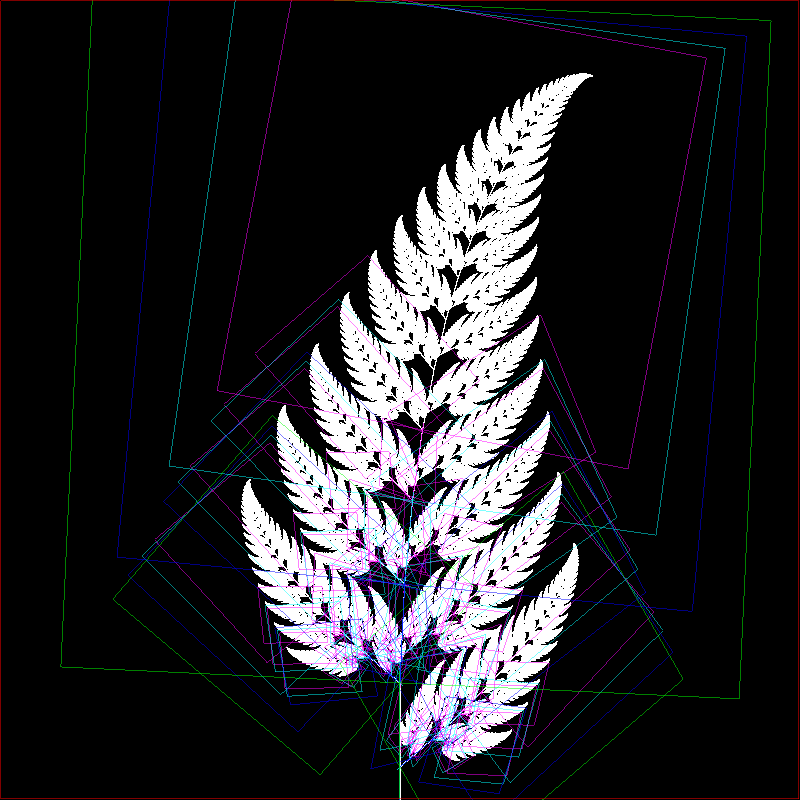
\includegraphics[width=\textwidth]{figures/barnsley_guides_and_points}
         \caption{guides and points}
         \label{figure:barnsley_guides_and_points}
     \end{subfigure}
     \hfill
     \begin{subfigure}[b]{0.3\textwidth}
         \centering
         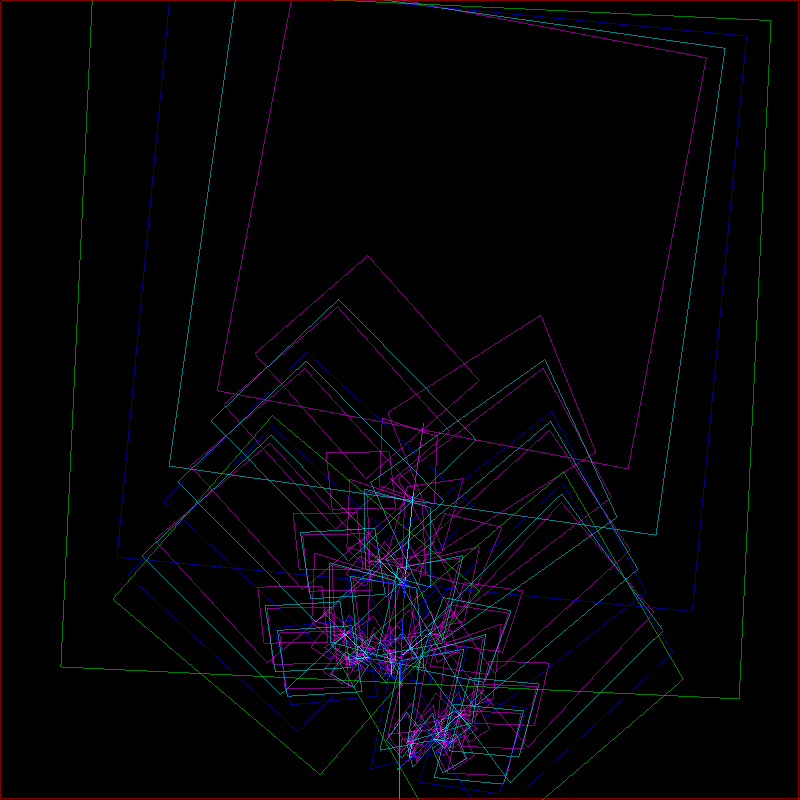
\includegraphics[width=\textwidth]{figures/barnsley_guides}
         \caption{only guides}
         \label{figure:barnsley_guides}
     \end{subfigure}
        \caption{The Barnsley Fern (\autoref{ifs:barnsley_fern}) rendered by the program in different ways.}
        \label{figure:barnsley_guides_vs_points}
\end{figure}

\section{Findings}
\label{sec:org4136bac}
\label{section:findings}

\subsection{Restrictions on replacing the view with a more shallow view}
\label{sec:org6f088f2}
\label{subsection:jumping_restrictions}

From experimentation with the program it turns out that there are two common situations
in which the technique of replacing the camera viewport with a more shallow camera viewport that is outlined in \autoref{subsection:self_similarity} cannot be used.

\begin{enumerate}
\item Borders between transformations
\label{sec:org6681592}

It is rather common to zoom in on the borders between transformations, as this is often
where interesting visual details of the IFS might appear.

\todo[inline]{Reference to-be-written earlier algorithm}

However, the algortihm as outlined in [REF] is not able to handle borders between transformations,
thus making it useless in these scenarios.

\item Overlapping subtransformations
\label{sec:orgf2038ec}

A more shallow view of the attractor only shows the same as a deeper view when
there are no points transformed by another mapping that end up in the deeper view.

When there are points from another mapping in the current view, 
going to a more shallow view will make points 'disappear' from the perspective of the user.
In practice, this means that for many IFSs there are large regions in which the technique cannot be used at all.

Simple IFSs like the Sierpi$\backslash$'nsky Triangle (\autoref{ifs:sierpinsky}), in which transformations
do not overlap, do not exhibit this problem. 
Slightly more complicated IFSs like the Dragon Curve[REF] or the Barnsly Fern[REF] however do.
See \autoref{figure:dragon_curve_overlaps} for an graphical explanation.

This case is annoyingly common and there is no clear solution to alleviate this restriction.
What is more, it is not simple to check whether we are currently in a region that exhibits the problem,
as this would require evaluating the IFS itself.

It is possible to take a rough 'upper bound' estimate of the disallowed regions by keeping track, 
per mapping, where the unit square would end up after a couple of mappings with this mapping as last (i.e. most significant) one.


\begin{figure}
     \centering
     \begin{subfigure}[b]{0.4\textwidth}
         \centering
         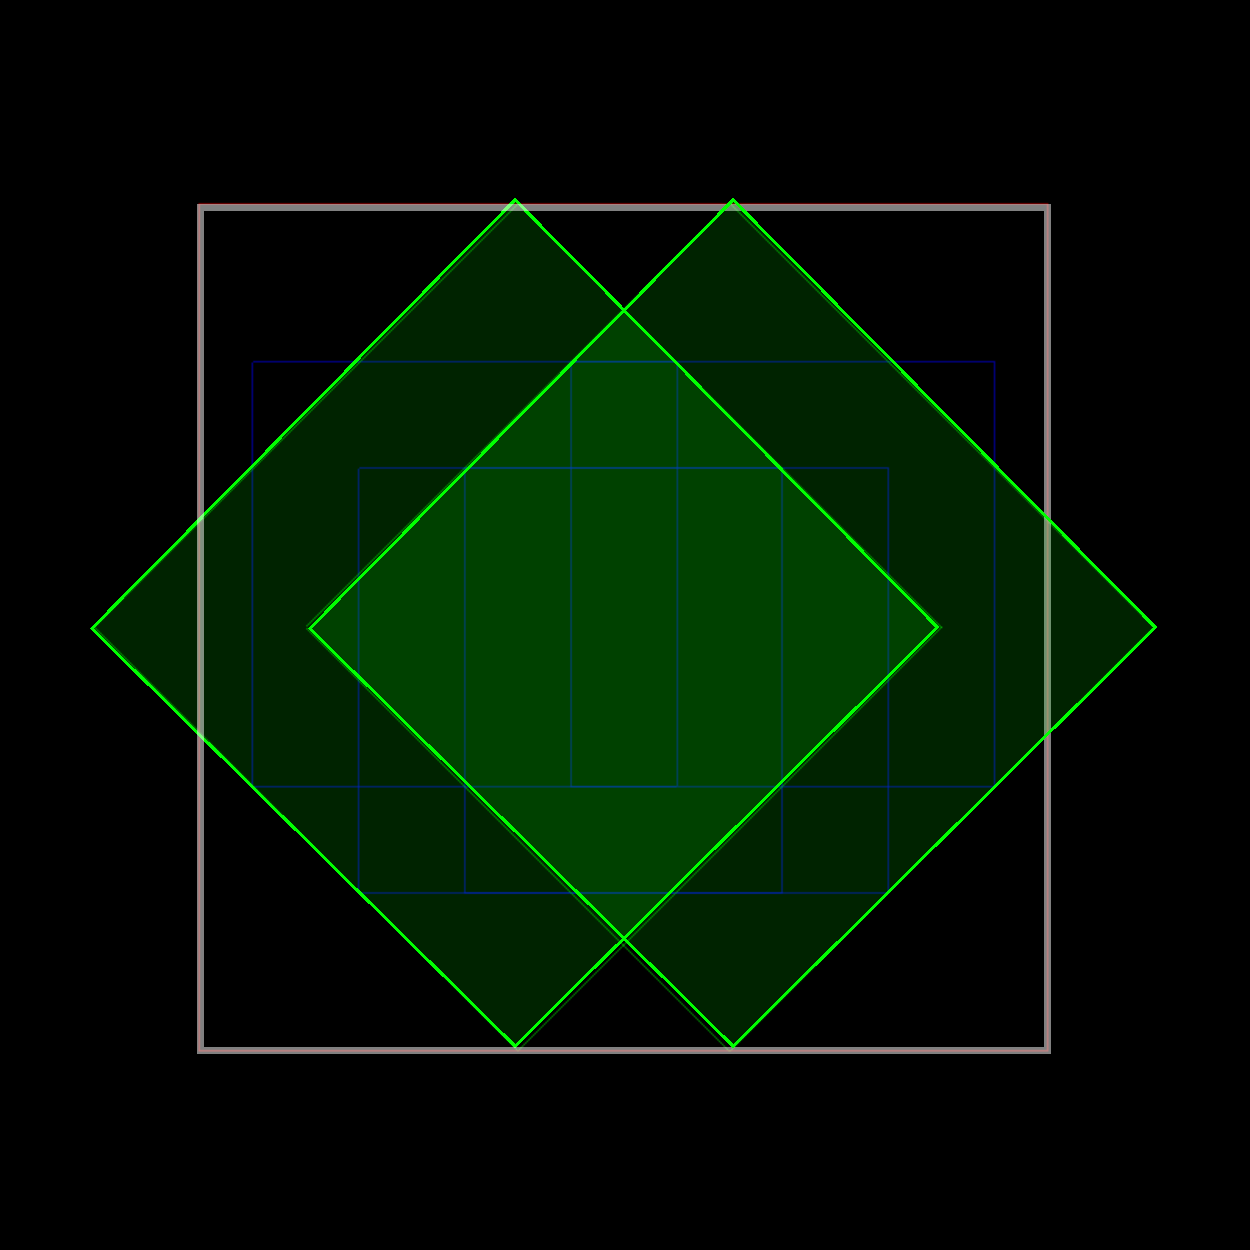
\includegraphics[width=\textwidth]{figures/dragon_curve_a}
         \caption{The unit square (indicated in white) transformed by the two mappings of $D$ (indicated in green)}
         \label{figure:dragon_curve_a}
     \end{subfigure}
     \hfill
     \begin{subfigure}[b]{0.4\textwidth}
         \centering
         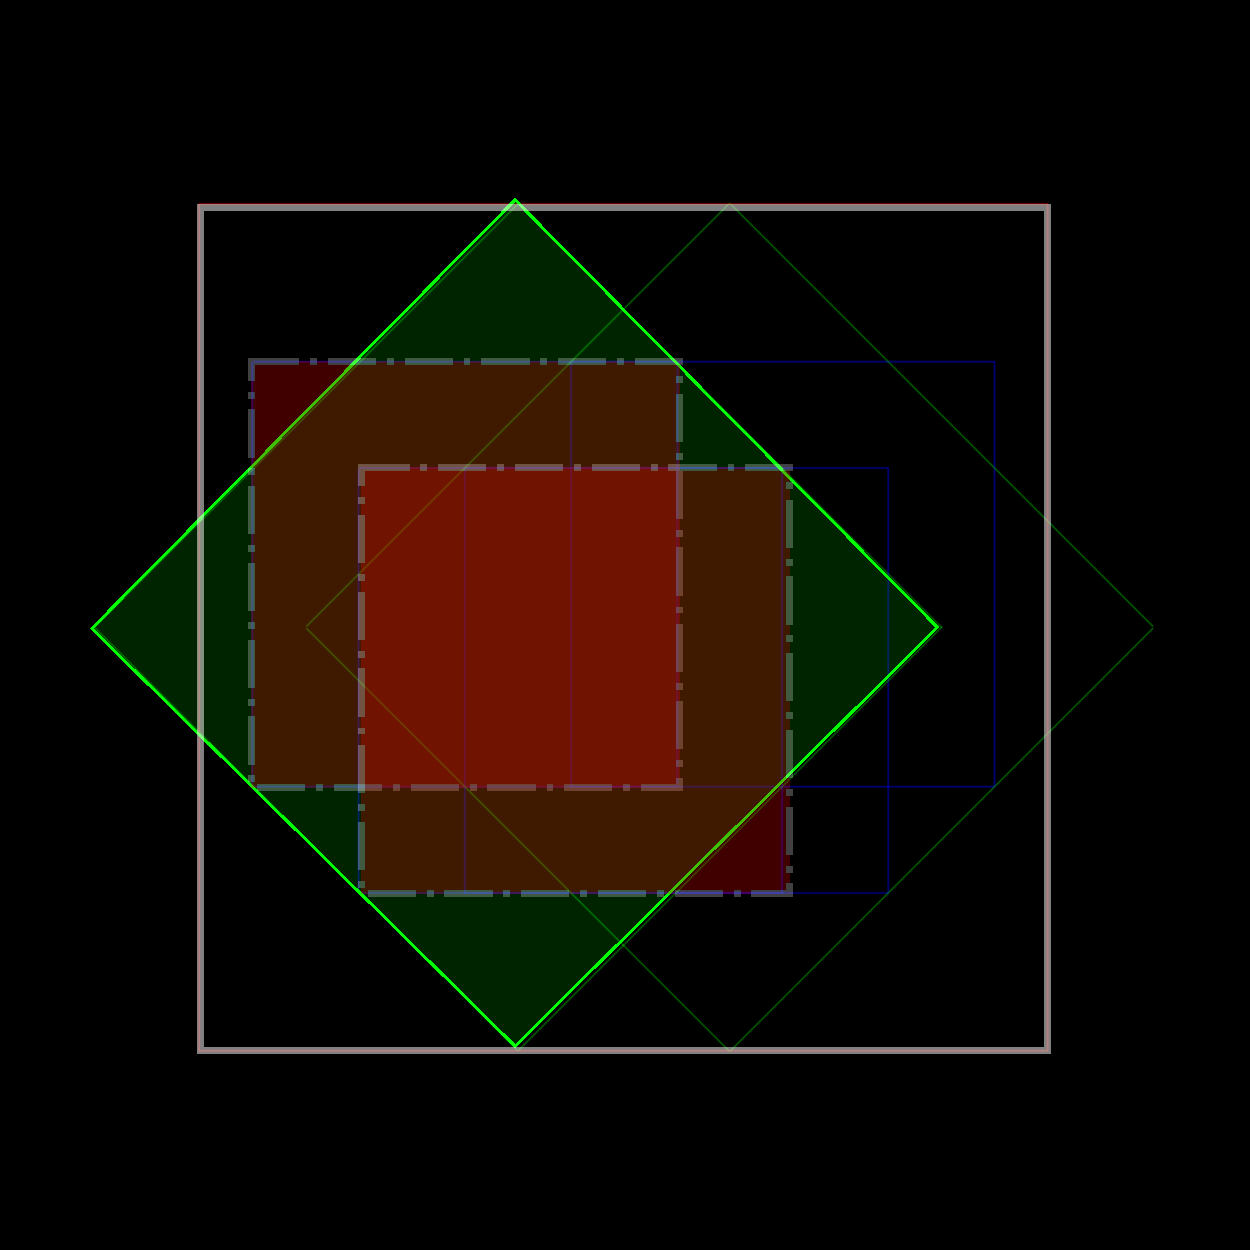
\includegraphics[width=\textwidth]{figures/dragon_curve_b}
         \caption{The first of the two mappings, transformed one more time by the mappings of $D$ (indicated in red)}
         \label{figure:dragon_curve_b}
     \end{subfigure}
     \hfill
     \begin{subfigure}[b]{0.4\textwidth}
         \centering
         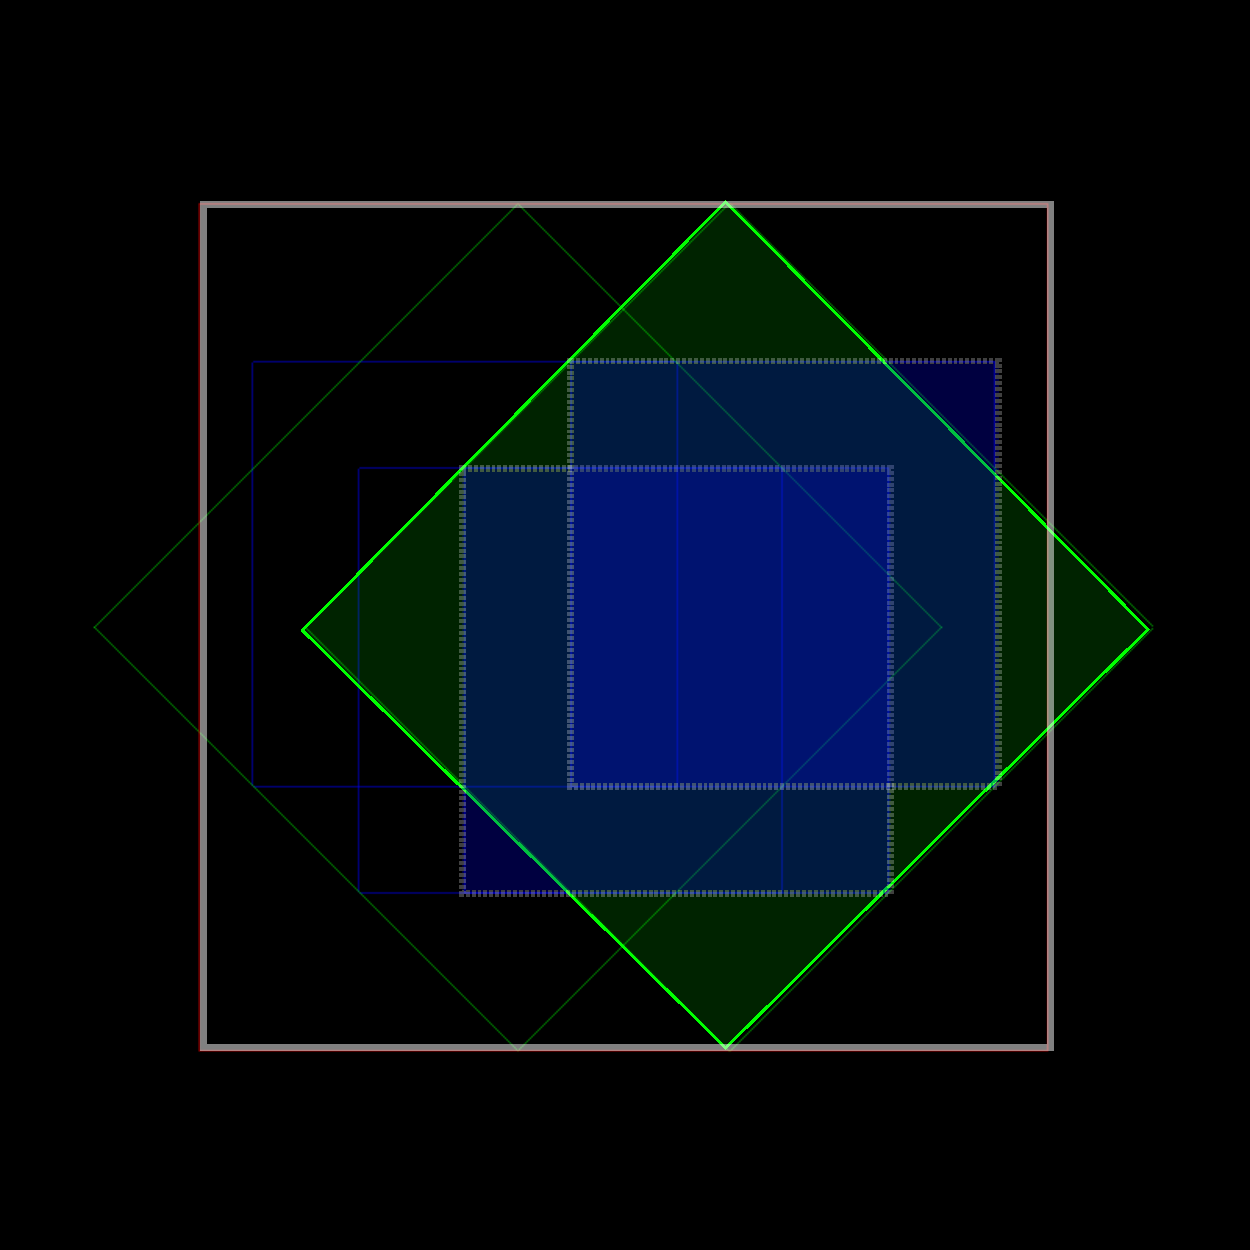
\includegraphics[width=\textwidth]{figures/dragon_curve_c}
         \caption{The second of the two mappings, transformed one more time by the mappings of $D$ (indicated in blue)}
         \label{figure:dragon_curve_c}
     \end{subfigure}
     \hfill
     \begin{subfigure}[b]{0.4\textwidth}
         \centering
         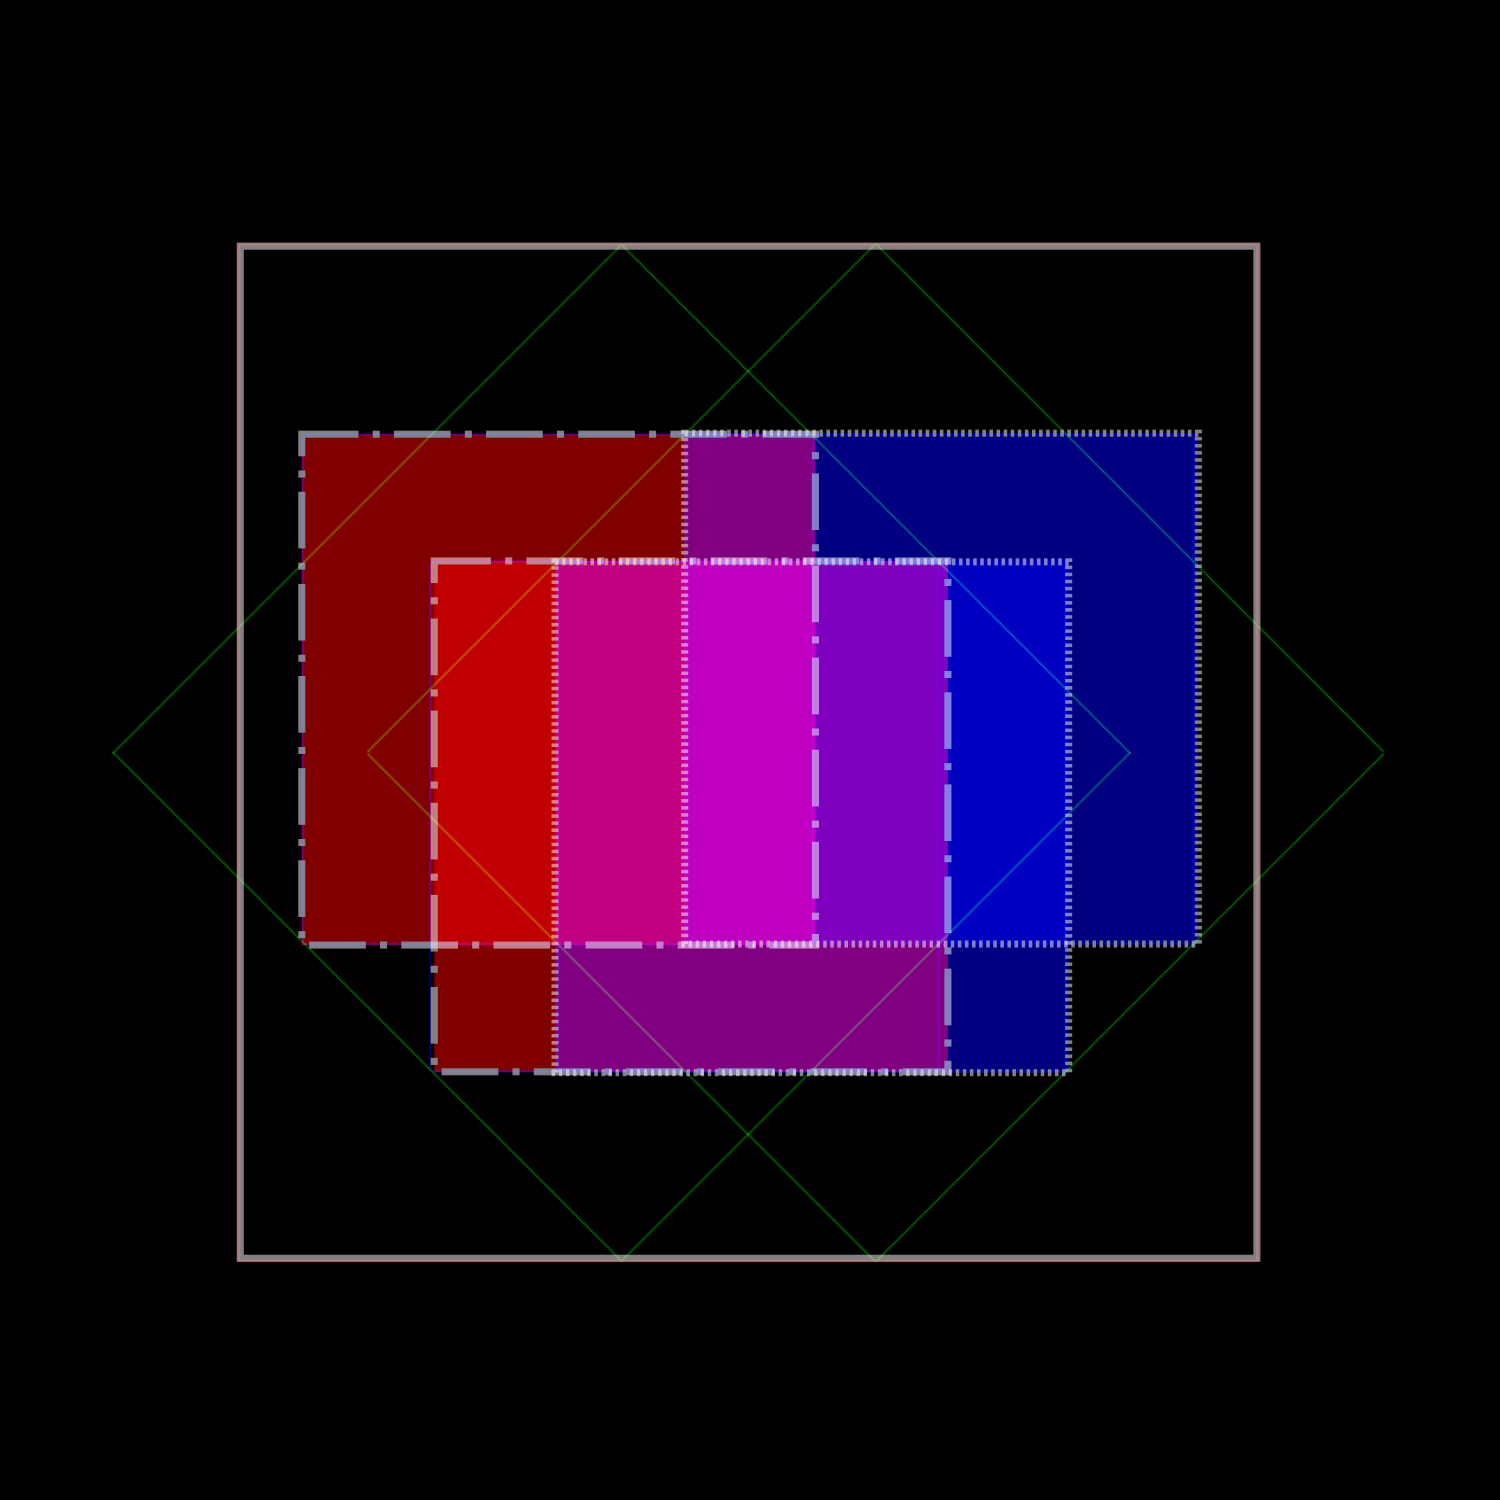
\includegraphics[width=\textwidth]{figures/dragon_curve_d}
         \caption{The region in which (b) and (c) overlap (indicated in magenta)}
         \label{figure:dragon_curve_d}
     \end{subfigure}
        \caption{Showing the first couple of iterations of rendering the attractor of the dragon curve IFS $D$ (\autoref{ifs:dragon_curve}), and the regions in which (sequences of) transformations overlap.}
        \label{figure:dragon_curve_overlaps}
\end{figure}

\todo[inline]{pseudocode}
\end{enumerate}

\subsection{Memory Usage}
\label{sec:org55cf330}

Point clouds take up a lot of data on the GPU. To render a fractal at reasonable detail, 
hundreds of millions if not billions of points are necessary (depending on the particular IFS).

A reasonable way to store a point cloud is by using for each 2D-point, 32 bits for each coordinate, thus fitting the pair in exactly one machine word of 64-bit systems.
Stored this way, a point cloud of 100,000,000 points requires 0.596 GiB of GPU memory,
and 1,000,000,000 points requires 5.96 GiB.
For current generation GPUs\footnote{At the time of writing, high-end consumer GPUs contain somewhere between 2 and 24 GiB of available memory. \cite{ign2020topgpus}}, this often is more memory than available.

\section{Conclusion}
\label{sec:orgea1fb94}
\label{section:conclusion}

A program was implemented which has shown that there is \emph{some} merit to rendering an IFS' attractor using a point-cloud as re-usable intermediate structure.
However, the self-similarity detection method that was proposed turns out to be unusable in common cases.
Furthermore, self-similarity 'jumps' make more sophisticated rendering techniques difficult if not impossible to use.

As long as these two problems remain unsolved, the proposed technique can only be considered impractical.

\section{Further Work}
\label{sec:org5966c97}
\label{section:further_work}

It is our hope that a more sophisticated way of detecting self-similarity might be found,
which would make 'self-similarity jumping' more practical.

Besides this, while we have shown in a proof-of-concept program that it is possible to render an IFS using a point cloud
with a reasonable speed, there are many optimizations that could be made to make the program run faster (potentially even in real-time),
most notably the rendering optimizations listed in \autoref{subsection:point_cloud_optimizations}

Another venue that could be explored is the rendering of an IFS' attractor at multiple 'levels of detail':
It might be possible to create more detailed local versions of the point cloud (based on the points of the less detailed point cloud) when the user
zooms in on a particular region, on demand.

Finally it is worth noting that as mentioned in \autoref{subsection:deterministic_gpu}, \cite{lawlor2012gpu} already presents an efficient way to render a large set of IFSs using a very different approach, 
which might be worthwhile to explore further.

\pagebreak
\printbibliography
\clearpage

\appendix

\section{IFSs used}
\label{sec:org9de4cd9}

This appendix lists the transformation matrices of the IFSs that were used throughout this thesis.

\todo[inline]{Sierpi\'nsky}
\todo[inline]{Dragon Curve}
\todo[inline]{Barnsley Fern}


\begin{ifs}
$$ 
\begin{aligned}
f_1(x, y) &= \begin{pmatrix} \frac{1}{2} & 0 \\ 0 & \frac{1}{2} \end{pmatrix} \begin{pmatrix} x \\ y \end{pmatrix} \\
f_2(x, y) &= \begin{pmatrix} \frac{1}{2} & 0 \\ 0 & \frac{1}{2} \end{pmatrix} \begin{pmatrix} x \\ y \end{pmatrix} + \begin{pmatrix} \frac{1}{2} \\ 0 \end{pmatrix} \\
f_3(x, y) &= \begin{pmatrix} \frac{1}{2} & 0 \\ 0 & \frac{1}{2} \end{pmatrix} \begin{pmatrix} x \\ y \end{pmatrix} + \begin{pmatrix} \frac{1}{4} \\ \frac{\sqrt{3}}{4} \end{pmatrix} \\
\end{aligned}
$$

\caption{the Sierpi\'nsky triangle or gasket}
\label{ifs:sierpinsky}
\end{ifs}

\begin{ifs}
$$ 
\begin{aligned}
f_1(x,y) &= \frac{1}{\sqrt{2}}\begin{pmatrix} \cos 45^\circ & -\sin 45^\circ \\ \sin 45^\circ & \cos 45^\circ \end{pmatrix} \begin{pmatrix} x \\ y \end{pmatrix}  \\
f_2(x,y) &= \frac{1}{\sqrt{2}}\begin{pmatrix} \cos 135^\circ & -\sin 135^\circ \\ \sin 135^\circ & \cos 135^\circ \end{pmatrix} \begin{pmatrix} x \\ y \end{pmatrix} + \begin{pmatrix} 1 \\ 0 \end{pmatrix} \\
\end{aligned}
$$

\caption{the Heighway Dragon Curve}
\label{ifs:dragon_curve}
\end{ifs}

\label{ifs:barnsley_fern}
\end{document}